\section{Results}

We fitted $7$ models with our methodology for each of our two outcome variables constructed based on the first user who used either the coin name or symbol in an ANN tagged thread.
Tables 1 and 2 report the coefficient estimates for standardized variables (both outcomes and measures have been linearly transformed to have mean 0 and standard deviation 1).
As a robustness check in the appendix tables 3 and 4 show the same results when applied to a 

Our User model considers how long a user has been active, and how many users have replied to them and he has replied to. 
Our nontrivial model consists of a single binary variable encoding wether the source code of the coin is a not a trivial change to existing coins. 
Our Satoshi model considers the distance and pagerank relative to satoshi.
None  of these three models achieve out of sample error rates beyond simply predicting $0$ constantly for either of our outcome measures of interest.


Our Network model encodes directed edges when a user interacts with another, and proceeds to estimate closeness centrality and clustering measures based on this. 
Our Weighted model uses the intensity of interactions to create a weighted network and construct a similar set of measures to the Network model.
Our interaction model includes interaction terms between non-trivialness and the weighted network measures.
Our All model contains all previous mentioned variables, there is extreme collinearity in this model and thus it's estimated coefficients and standard errors should be interpreted with extreme caution. 


\begin{figure}[h]
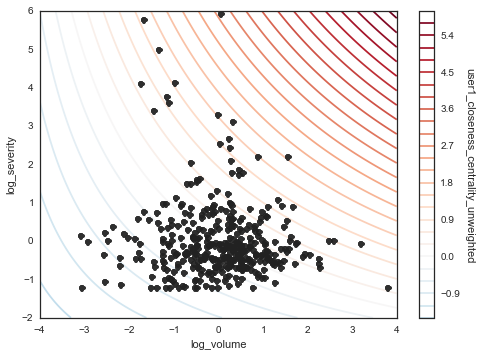
\includegraphics[width=\columnwidth]{centrality_volume_severity}
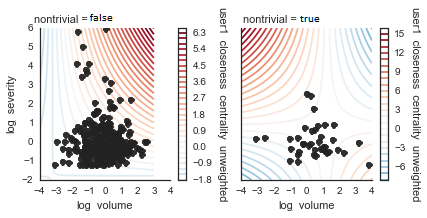
\includegraphics[width=\columnwidth]{centrality_volume_severity_nontrivial}
\end{figure}

The main driver of our explanatory power is the centrality of a user in the directed network derived from the forum. 
This effect appears to be mediated by whether a coin involves a nontrivial technological change, the direction of the interaction reversing depending on whether it relates to magnitude or severity.
While the linear model is not able to fully capture this interaction, plotting the values of severity and magnitude of bubbles and the centrality reveals a interaction; with the polarity of the gradients flipping in the severity case.

%JULIAN: Above sentence is tough to parse, but kind of an important one.
Both the severity and the magnitude of bubbles increases with the centrality of the user who introduces the coins in the forums.  
Interestingly this effect is concentrated in different ways depending on whether the coin software is more than a trivial modification: trivial coins have more severe bubbles the more central their introducers are, while volume is greater the more central the introducer of a nontrivial coin is.






\begin{figure}[h]
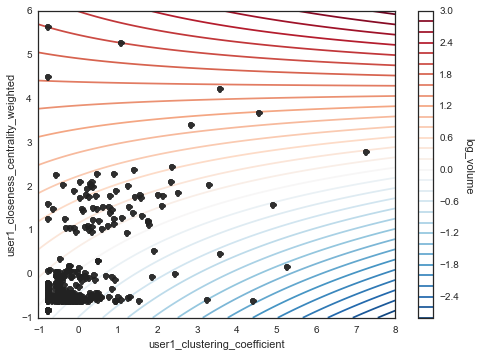
\includegraphics[width=\columnwidth]{cluster_closeness_volume}
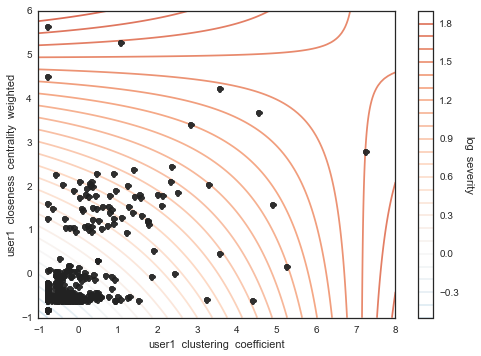
\includegraphics[width=\columnwidth]{cluster_closeness_severity}
\end{figure}

